\seite{}{Lattice-Boltzmann}\anchorpage{1}{neu8}{8 · Mesoskopische Strömungssimulation mit der Lattice-Boltzmann-Methode}\ey{KAPITEL 8}\ptitle{Mesoskopische Strömungssimulation mit der Lattice-Boltzmann-Methode}
Der Deckel schiebt die oberste Flüssigkeitsschicht nach rechts. Weiter unten beginnt das Fluid erst später zu kreisen. Ein Gitterpunkt kann die Bewegung seiner Nachbarn weitergeben, obwohl er nur eine Handvoll Zahlen speichert. Welche Information müssen diese Zahlen tragen, damit aus ihren Verschiebungen Dichte, Impuls und ein Wirbel entstehen?
\subt{Der Weg durch das Kapitel}
{\tblstart\begin{tabularx}{\linewidth}{@{}Yr@{}}\toprule
\hyperlink{abs8-1}{8.1 · Von der kinetischen Beschreibung zur Strömung} & \pagelink{abs8-1}\\[2pt]
\hyperlink{abs8-2}{8.2 · Das D2Q9-Gittermodell} & \pagelink{abs8-2}\\[2pt]
\hyperlink{abs8-3}{8.3 · Kollision und Streaming} & \pagelink{abs8-3}\\[2pt]
\hyperlink{abs8-4}{8.4 · Wände und Einheiten} & \pagelink{abs8-4}\\[2pt]
\bottomrule\end{tabularx}\par}
\par\vfill{\centering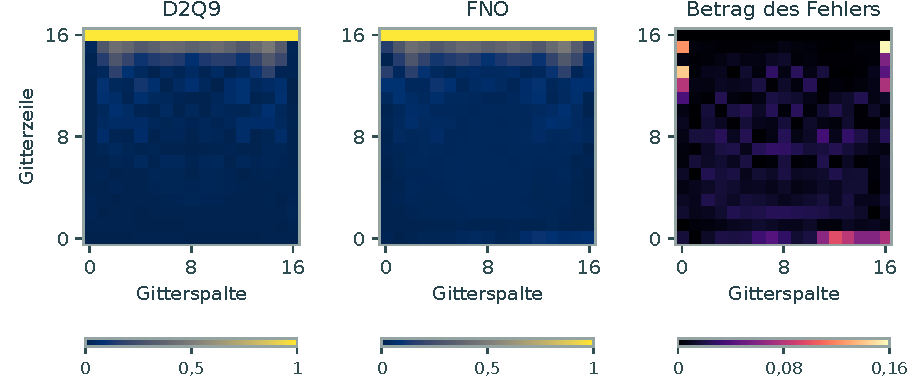
\includegraphics[width=.88\linewidth,height=49mm,keepaspectratio]{cp2kavitaet.pdf}\par}\capline{Der bewegte Deckel setzt das Innere der Kavität in Bewegung.}
\seite{}{Lattice-Boltzmann}\anchorpage{2}{abs8-1}{8.1 · Von der kinetischen Beschreibung zur Strömung}\ey{ABSCHNITT 8.1}\ptitle{Von der kinetischen Beschreibung zur Strömung}
\hypertarget{punkt8-1-1}{}\subt{8.1.1\enspace Verteilungen über Geschwindigkeiten}
Stellen Sie sich eine kleine Messzelle vor. Zwei Teilchenpakete können gleich viel Masse enthalten und doch mit sehr verschiedenen Geschwindigkeiten eintreffen. Die Verteilung \(f(x,\xi,t)\) beschreibt, wie viel Masse am Ort \(x\) einer Geschwindigkeit \(\xi\) zugeordnet ist. Ohne äußere Kraft lautet ihre Transportgleichung \(\partial_t f+\xi\cdot\nabla_x f=\Omega(f)\). Freier Transport verschiebt die Verteilung, Stöße verändern ihre Form.
\hypertarget{punkt8-1-2}{}\subt{8.1.2\enspace BGK-Relaxation und hydrodynamische Grenze}
BGK ersetzt den komplizierten Stoßoperator durch \(-(f-f^{eq})/\tau_{phys}\). Kleines positives \(\tau_{phys}\) führt rasch zum örtlichen Gleichgewicht. Dichte und Impuls sind die niedrigsten Momente. Unter geeigneter Skalierung, kleinen Knudsen- und Mach-Zahlen und hinreichender Gitterisotropie liefern ihre Bilanzen die makroskopische Strömungsdynamik. Der folgende Gitteralgorithmus benutzt eine dimensionslose Relaxationszeit in Schritten.
\seite{}{Lattice-Boltzmann}\anchorpage{2}{abs8-2}{8.2 · Das D2Q9-Gittermodell}\ey{ABSCHNITT 8.2}\ptitle{Das D2Q9-Gittermodell}
\hypertarget{punkt8-2-1}{}\subt{8.2.1\enspace Neun Richtungen und ihre Gewichte}
In der Mitte bleibt ein Anteil liegen, vier ziehen längs der Achsen, vier diagonal. Die Gewichte betragen \(4/9,1/9,1/36\) je Richtung der jeweiligen Gruppe. Ihre Summe ist eins. Gegenrichtungen wie Ost und West heben sich im ersten Moment eines ruhenden Gleichgewichts auf. In Gittereinheiten gilt \(c_s^2=1/3\).
\hypertarget{punkt8-2-2}{}\subt{8.2.2\enspace Das diskrete Gleichgewicht bei kleiner Mach-Zahl}
Eine Entwicklung der Maxwell-Verteilung bis zum Quadrat in \(u\) liefert
\[
 f_i^{eq}=w_i\rho\left(1+\frac{c_i\cdot u}{c_s^2}
 +\frac{(c_i\cdot u)^2}{2c_s^4}-\frac{u\cdot u}{2c_s^2}\right).
\]
Dreht sich das Fluid nach Osten, wächst die ostwärts gerichtete Population relativ zur westwärts gerichteten. Die quadratischen Terme sorgen für das passende zweite Moment im Arbeitsbereich der Näherung.
\hypertarget{punkt8-2-3}{}\subt{8.2.3\enspace Dichte, Impulsdichte und Impulsfluss}
Ohne äußere Kraft gilt \(\rho=\sum_i f_i\) und \(\rho u=\sum_i c_i f_i\). Der Impulsfluss ist der Tensor \(\Pi=\sum_i(c_i\otimes c_i)f_i\). Schon die Einheiten unterscheiden Masse pro Volumen, Impuls pro Volumen und Impulstransport über eine Fläche. Im Labor ändern wir die Populationen bei unveränderten ersten beiden Momenten.
\lektion{Neun Zahlen in einer einzigen Zelle}{zellenlbm}{Rechenversuch}{Lattice-Boltzmann}
\lernziel{Sie können vorhersagen, wie eine Lattice-Boltzmann-Zelle auf eine kleine Störung reagiert und was die Nachbarzelle im nächsten Schritt erhält.}
Die Einträge \(f_i\) verteilen die lokale Dichte auf mögliche Bewegungsrichtungen. Für Flüssigkeit in Ruhe bei \(\rho=1\) hat der D2Q9-Gleichgewichtszustand in Gittereinheiten die folgenden Werte.
{\tblstart\begin{tabularx}{\linewidth}{@{}Yrr@{}}\toprule
\hd{Richtung}&\hd{Anzahl}&\hd{Wert je Richtung}\\\midrule
Ruhe, \(\mathbf c=(0,0)\)&1&4/9\\
Ost, Nord, West, Süd&4&1/9\\
Diagonalen&4&1/36\\\bottomrule
\end{tabularx}\par}
Die Dichte ist \(4/9+4/9+4/36=1\). Gegenüberliegende Richtungen haben gleiches Gewicht. Ihre Impulse heben sich auf, also ist die mittlere Geschwindigkeit null. In einer gleichmäßig ruhenden Flüssigkeit wiederholt sich dieser Zustand nach Kollision und Transport.
\subt{Ein Schritt außerhalb des Gleichgewichts}
Geben Sie Ost und West je \(0{,}02\) zusätzlich und nehmen Sie dem Ruheanteil \(0{,}04\) weg. Dichte und Impuls bleiben gleich. Trotzdem hat sich der Zustand geändert. Wählen wir für die Handrechnung \(\omega=1/2\), halbiert die BGK-Kollision jede Abweichung vom Gleichgewicht. Der Ostanteil geht von \(1/9+0{,}02=0{,}131111\ldots\) auf \(1/9+0{,}01=0{,}121111\ldots\) zurück. Der Ruheanteil bleibt um \(0{,}02\) unter \(4/9\).

Beim anschließenden Transport wandert der neue Ostanteil in die östliche Nachbarzelle. Dort muss seine Dichtewirkung mit den acht anderen ankommenden oder ruhenden Anteilen zusammengezählt werden. Erst daraus lässt sich eine Geschwindigkeit an diesem Ort bestimmen. Am Deckel greift zusätzlich die vorgeschriebene Randregel.
\notebox{Probe}{Welchen Unterschied hätte eine einzige gespeicherte Geschwindigkeit vor der Kollision gezeigt? Beide Zustände haben Geschwindigkeit null. Die neun gespeicherten Anteile bewahren zusätzlich das Richtungsungleichgewicht.}
\srcs{\href{https://benchpress.readthedocs.io/autodoc_benchmarks/lattice_boltzmann_D2Q9.html}{D2Q9-Gewichte im Rechenbeispiel von Jonas Latt} · \texttt{python methodenlabor.py} · \see{schluss13}{Lokaler Erhaltungsbeweis}.}

\seite{}{Lattice-Boltzmann}\anchorpage{2}{abs8-3}{8.3 · Kollision und Streaming}\ey{ABSCHNITT 8.3}\ptitle{Kollision und Streaming}
\hypertarget{punkt8-3-1}{}\subt{8.3.1\enspace Lokale Kollision}
Alle neun Eingangswerte stammen aus der gleichen Zelle. Nach der Momentenbildung berechnet man \(f_i^*=f_i-(f_i-f_i^{eq})/\tau\). Für \(\tau=2\) halbiert die Kollision jede Abweichung vom aktuellen Gleichgewicht. Die Ausgangswerte gehören weiter zur selben Zelle.
\hypertarget{punkt8-3-2}{}\subt{8.3.2\enspace Transport in den Nachbarpuffer}
Mit Gitterzeit eins schreibt Streaming \(f_i(x+c_i,t+1)=f_i^*(x,t)\). Eine doppelte Pufferung verhindert, dass ein frisch geschriebener Wert im selben Takt ein zweites Mal reist. Gegenprobe mit einem einzigen markierten Ostanteil: Nach einem Takt muss der Wert genau eine Spalte weiter im Ostkanal erscheinen.
\hypertarget{punkt8-3-3}{}\subt{8.3.3\enspace Beweis der lokalen Erhaltung}
Die D2Q9-Symmetrien liefern \(\sum w_i=1,\ \sum w_ic_i=0,\ \sum w_ic_ic_i^T=c_s^2I\), und alle ungeraden dritten Momente verschwinden. Einsetzen in das Gleichgewicht ergibt \(\sum f_i^{eq}=\rho\) und \(\sum c_if_i^{eq}=\rho u\). Daher haben die Kollisionskorrekturen sowohl Summe als auch erstes Moment null. Beim Streaming wandert Masse zwischen den Zellen. Eine periodische Gesamtbilanz bleibt erhalten, eine bewegte Wand kann Impuls zuführen.
\seite{}{Lattice-Boltzmann}\anchorpage{2}{abs8-4}{8.4 · Wände und Einheiten}\ey{ABSCHNITT 8.4}\ptitle{Wände und Einheiten}
\hypertarget{punkt8-4-1}{}\subt{8.4.1\enspace Bounce-back an einer ruhenden Wand}
Eine Population, die im nächsten Schritt in eine feste Wand liefe, kehrt in die Gegenrichtung zurück. Vollweg- und Halbweg-Varianten verorten die Rückgabe unterschiedlich. Damit ändern sich die effektive Wandlage und möglicherweise die Konvergenz. Die Lage des geometrischen Randes gehört deshalb zum Vergleich zweier Gitter.
\hypertarget{punkt8-4-2}{}\subt{8.4.2\enspace Geschwindigkeitsrand und bewegter Deckel}
Bei Zou–He werden fehlende einlaufende Populationen aus den Zielmomenten und einer Schließungsannahme für den Nichtgleichgewichtsanteil rekonstruiert. Nach diesem Update müssen Normalmassenstrom und gewünschte Tangentialgeschwindigkeit zusammenpassen. CP2 benutzt im hier reproduzierten Algorithmus Vollweg-Reflexion an ruhenden Wänden und vorgegebene Gleichgewichtspopulationen an der Deckelzeile. Ein Wechsel der Randvorschrift ist ein neuer Versuch.
\hypertarget{punkt8-4-3}{}\subt{8.4.3\enspace Physikalische und Gittereinheiten}
Bei Gitterweite \(\Delta x\) und Zeittakt \(\Delta t\) gilt \(u_{lat}=u_{phys}\Delta t/\Delta x\), \(\nu_{lat}=\nu_{phys}\Delta t/\Delta x^2=c_s^2(\tau-1/2)\). Die Reynolds-Zahl \(UL/\nu\) bleibt unter konsistenter Umrechnung gleich. Positive BGK-Viskosität erfordert \(\tau>1/2\). Für einen belastbaren Lauf prüfen wir außerdem Mach-Zahl, Massenbilanz und die Mittellinienprofile.
\srcs{\href{https://arxiv.org/abs/comp-gas/9611001}{Zou und He, Geschwindigkeits- und Druckränder} · \see{pylbm}{CP2-Kavität}.}
\lektion{Eine D2Q9-Zelle Schritt für Schritt}{alg8}{Werkstatt}{Kapitel 8}
Zwei Gitterpuffer trennen ankommende Populationen von gerade fortgeschriebenen. Beim Streaming muss eine nach Osten auslaufende Population der westlichen Nachbarzelle im Ostkanal der Zielzelle erscheinen.
{\small\begin{verbatim}
fuer jede Zelle x:
    rho = summe(f[x])
    u = impuls(f[x]) / rho
    fuer jede Richtung i:
        eq = gleichgewicht(i, rho, u)
        stern[x,i] = f[x,i] - (f[x,i] - eq) / tau
fuer jede fluide Verbindung (x, i):
    neu[x + c[i], i] = stern[x, i]
behandle_Wandverbindungen_nach_der_Randregel()
\end{verbatim}}
\subt{Selbst rechnen}
Ein ruhendes Gitter besitzt je Zelle Dichte eins. Ost und West erhalten jeweils 0,02 zusätzlich, vom Ruheanteil werden 0,04 abgezogen. Wie sieht die Störung nach einer BGK-Kollision bei \(\tau=2\) aus?
\notebox{Lösung}{Dichte und Impuls bleiben unverändert. Dadurch bleibt auch das Gleichgewicht gleich. Der Kollisionsschritt halbiert jede Abweichung, also +0,01 im Ost- und Westkanal und \ensuremath{-}0,02 im Ruhekanal. Erst das Streaming verteilt diese Störung auf Nachbarn.}
